\chapter{Laboratorio 1}
In questa esperienza di laboratorio si è realizzato e analizzato il seguente circuito:
\begin{figure}[h!]
	\centering
	\begin{minipage}{.4\textwidth}
	\scalebox{.835}{
		\begin{circuitikz}
			\draw (0,.5) node[ground]{};
			\draw (0,2) to[sV=$v_{in}$] (0,.5);
			\draw (0,2) to[R=$R_2$, -*] ++(3,0) ++(0.1,-.1) node[below]{$V^-$};
			\draw (3,2) to (4,2);
			\draw (3.7,2) node[op amp, anchor=-](oa){\texttt{TL071}};
			\draw (oa.up) -- ++(0, 0.3) node[vcc]{$+E$};
			9 \draw (oa.down) -- ++(0,-0.3) node[vee]{$-E$};
			\draw (3.7,.5) node[ground]{} to[short, -*] (3.7,1);
			\draw (3,2) -- ++(0,2.3) coordinate(C) to[C=$C_1$] ++(3.08,0) (C-|oa.out) coordinate(Co) -- (oa.out) to [short, *-o] ++(1,0) node[above]{$v_{out}$};
			\draw (3,4.3) -- ++(0,1.3) to[R=$R_1$] ++(3,0) -| (Co);
			\draw[thick] (-.7,-.5) rectangle (7.65,6.5);
		\end{circuitikz}
	}
	\end{minipage}
	\qquad\qquad
	\begin{minipage}{.5\textwidth}
		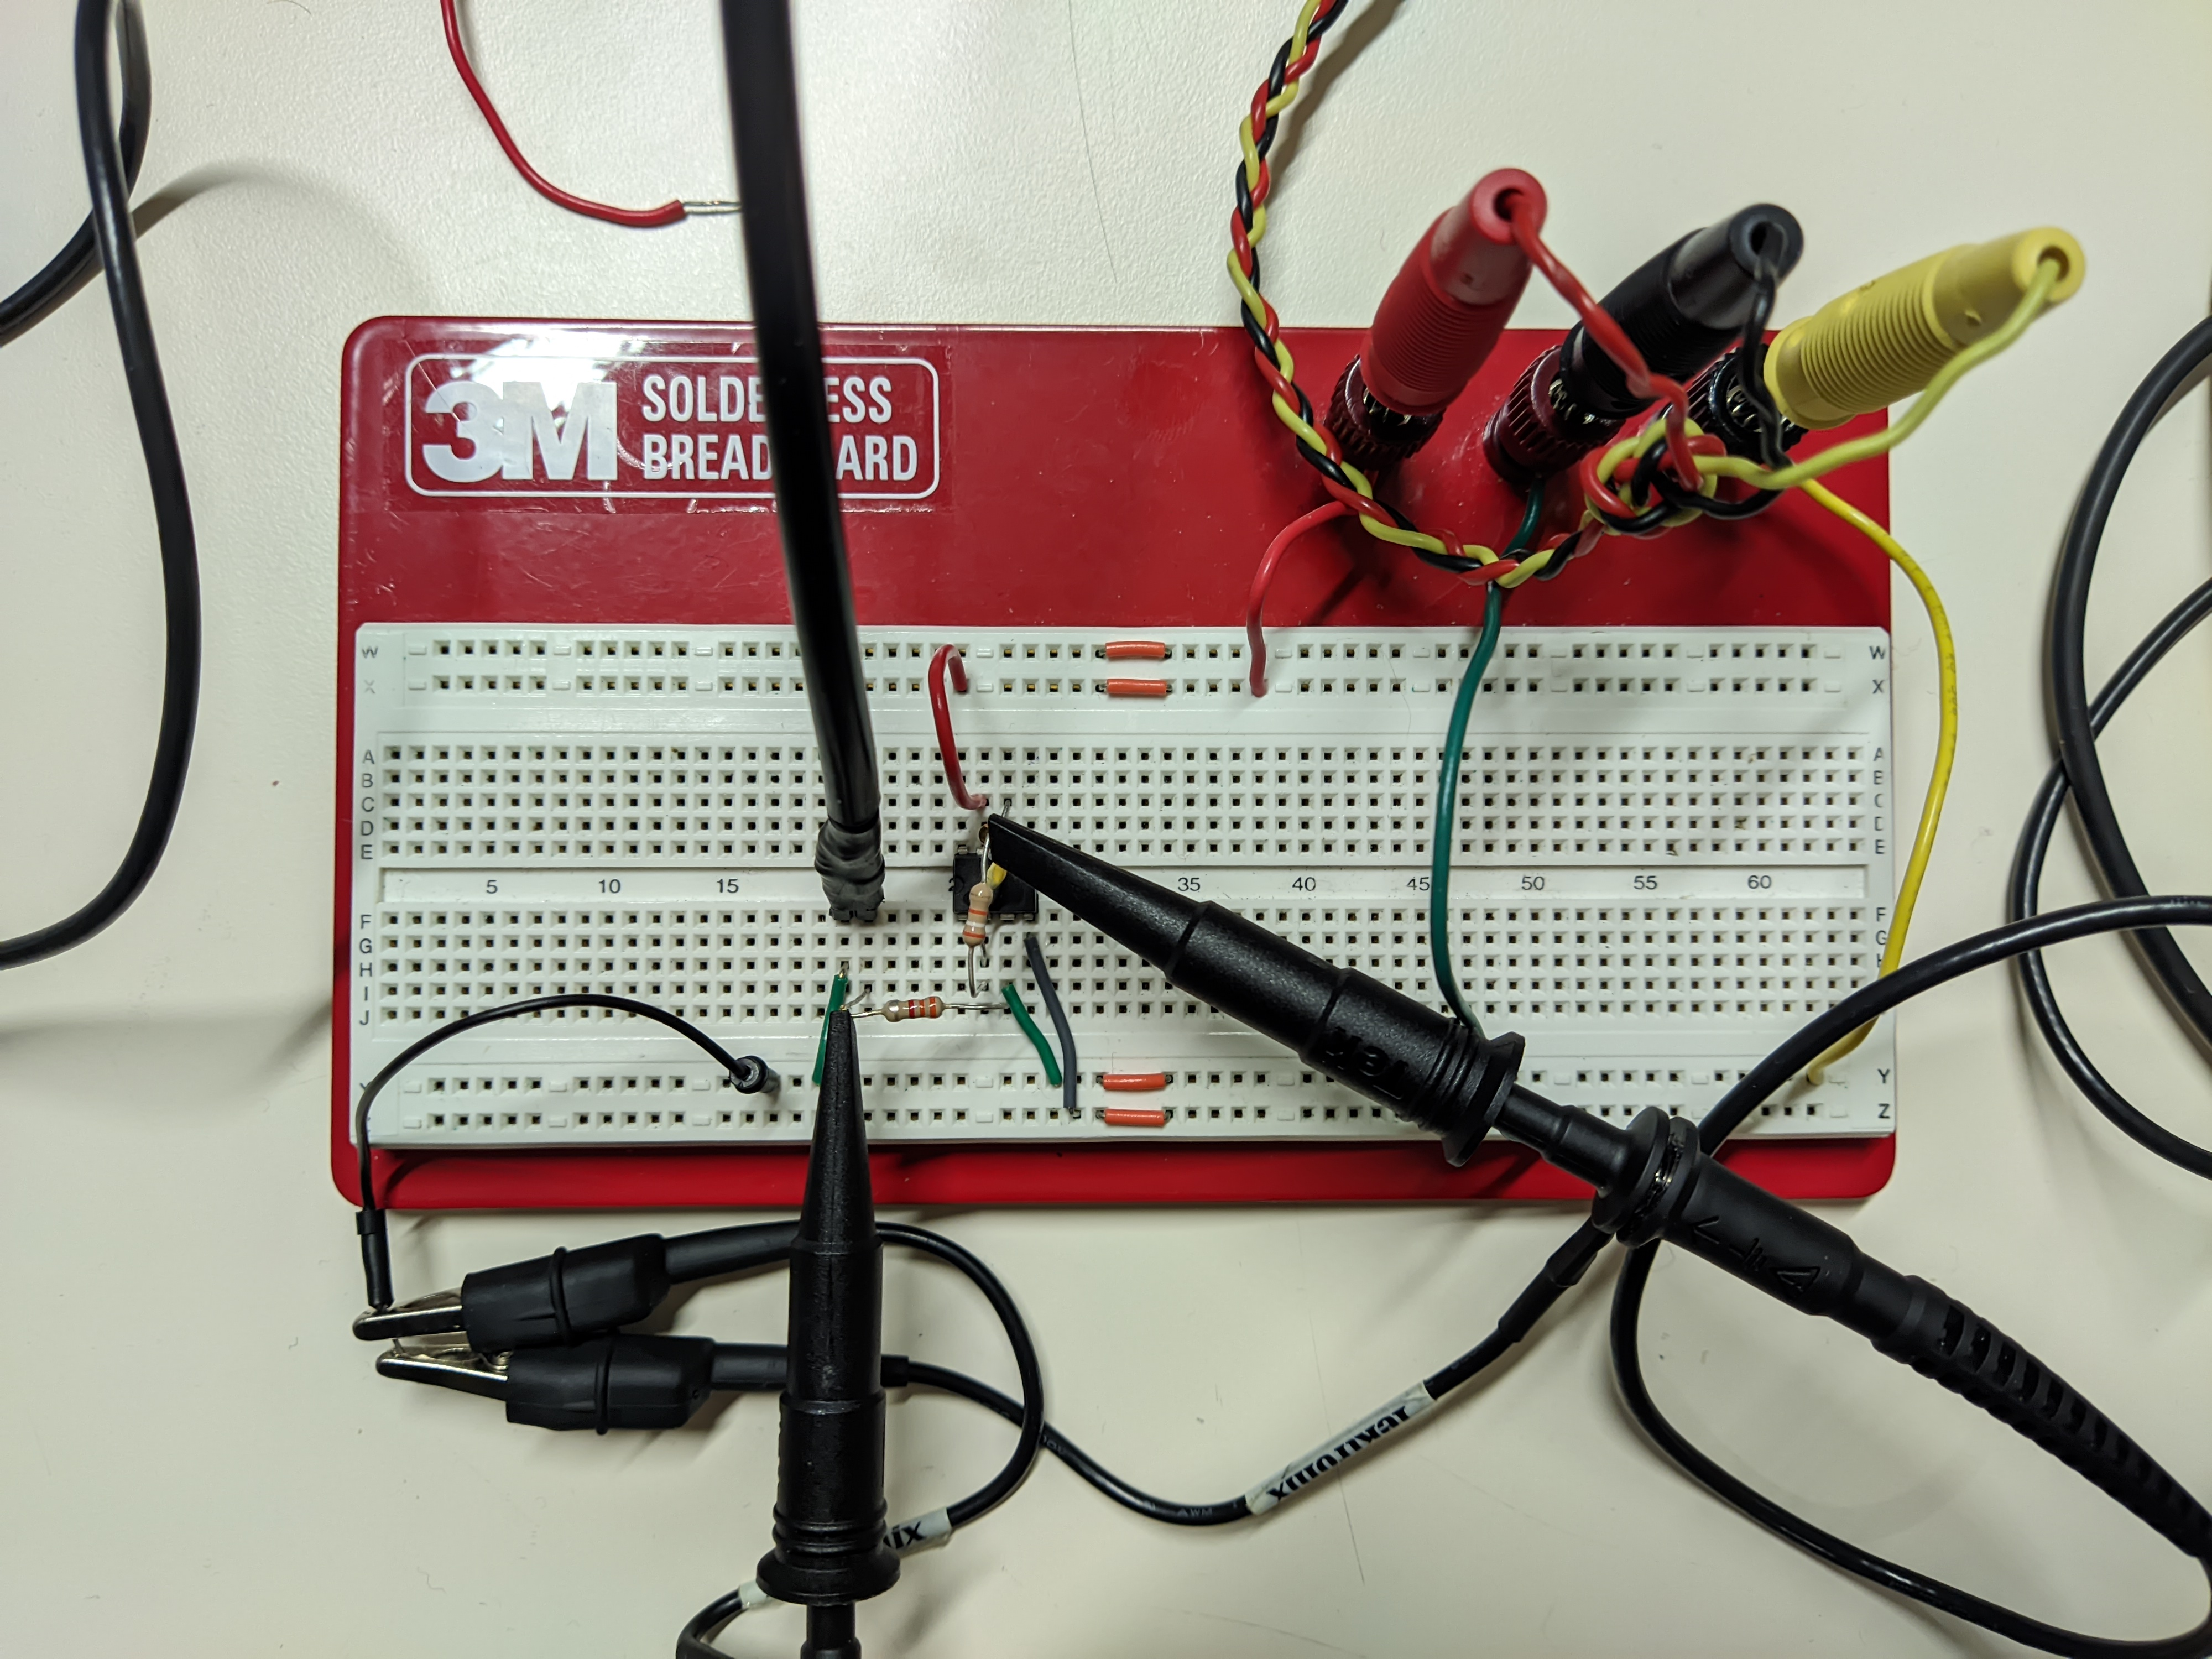
\includegraphics[width=\linewidth]{./ImageFiles/Laboratorio 1/CIRC.jpg}
	\end{minipage}
	\caption{Schema e foto del circuito realizzato.}
	\label{fig:circuito}
\end{figure}

\noindent
Il circuito realizza un filtro passa basso attivo del primo ordine, utilizzando un amplificatore operazionale retroazionato negativamente. In particolare, si utilizza l'amplificatore operazionale TL071 (\url{https://www.st.com/resource/en/datasheet/tl071.pdf}). Questo amplificatore rientra nella categoria degli operazionali \textit{general-purpose} ed è caratterizzato da elevati slew rate e basse correnti di ingresso.
\`E possibile ricavare la funzione di trasferimento del circuito tramite un bilancio delle correnti al nodo V\super{-}. Si consideri $v\sub{in}$ come un generatore ideale di tensione applicato in ingresso al circuito. Indicando con Z\sub{1} l'impedenza equivalente del parallelo tra R\sub{1} e C\sub{1} e con Z\sub{2} l'impedenza della resistenza R\sub{2}, si può ottenere la funzione di trasferimento del circuito:
\begin{equation}
	v_{out}=-\frac{Z_1}{Z_2}v_{in}=-\frac{R_1}{R_2}\frac{1}{1+j w R_1 C_1} v_{in},
\end{equation}
da cui si ricava
\begin{equation}
	T=\frac{v_{out}}{v_{in}}=-\frac{R_1}{R_2}\frac{1}{1+j w R_1 C_1}.
\end{equation}
Questa funzione di trasferimento corrisponde a quella di un filtro passa basso. È possibile calcolare il valore del modulo e della fase in funzione della pulsazione del segnale in ingresso $\omega$ tramite le seguenti espressioni:
\begin{equation}
	\begin{split}
		|T|&=\frac{R_1}{R_2}\frac{1}{\sqrt{1+(wR_1C_1)^2}} \\
		\angle T&=\SI{180}{\degree}-arctan(\omega R_1 C_1).
	\end{split}
	\label{eq:1.3}
\end{equation}
Per comprendere l'andamento del modulo e della fase in funzione della frequenza del segnale applicato in ingresso, è necessario analizzare i termini dipendenti da $\omega$ nelle due equazioni. Nell'espressione del modulo della funzione di trasferimento, il termine 
\begin{equation}
	\sqrt{1+(wR_1C_1)^2} \to
	\begin{cases}
		1 \; per \; \omega \to 0 \\
		\infty \; per \; \omega \to \infty
	\end{cases}
,
\end{equation}
mentre nell'espressione della fase, il termine
\begin{equation}
	arctan(\omega R_1 C_1) \to
	\begin{cases}
		0 \; per \; \omega \to 0 \\
		90^\circ \; per \; \omega \to \infty
	\end{cases}
	.
\end{equation}
Quindi il modulo tende a $\frac{R_1}{R_2}$ per segnali in ingresso a bassa frequenza, mentre tende a zero per segnali in ingresso ad alta frequenza. La fase, invece, è pari a circa \SI{180}{\degree} per segnali a bassa frequenza, e tende a \SI{90}{\degree} per segnali ad alta frequenza.
Il comportamento del circuito è quindi quello di un filtro passa basso invertente del primo ordine, con frequenza di taglio pari a $f=\frac{1}{2\pi R_1C_1}$.

\noindent
I valori dei componenti passivi sono stati scelti per soddisfare i requisiti di prestazioni del filtro. In particolare, veniva richiesto un guadagno di un fattore 10 con frequenza di taglio pari a \SI{10}{\kilo\hertz}. I valori nominali ed effettivi dei componenti passivi utilizzati sono riportati in tabella \ref{tab:valori_componenti}. Inoltre, le tensioni di alimentazione positiva +E e negativa -E dell'amplificatore operazionale sono state fissate rispettivamente a +\SI{10}{\volt} e -\SI{10}{\volt}.

\def\arraystretch{1.3}
\begin{table}[h]
	\centering
	\begin{tabular}{|c|c|c|}
		\hline
		Componente	& Valore Nominale & Valore Misurato \\ \hline
		R\sub{1}          & \SI{38}{\kilo\ohm} &     \SI{38.10}{\kilo\ohm}  \\ \hline
		R\sub{2}          & \SI{3.3}{\kilo\ohm} &      \SI{3.29}{\kilo\ohm} \\ \hline
		C\sub{1}          & \SI{390}{\pico\farad} &   Non misurato  \\ \hline
		
	\end{tabular}
	\caption{Valori nominali e misurati dei componenti passivi del circuito.}
	\label{tab:valori_componenti}
\end{table}

\noindent
Attraverso un generatore di forme d'onda sono stati applicati in ingresso al circuito dei segnali sinusoidali con ampiezza picco-picco pari a \SI{500}{\milli\volt} e frequenza compresa tra i \SI{100}{\hertz} e i \SI{10}{\mega\hertz}. Nella figura \ref{fig:misure_oscilloscopio_1} sono riportati i segnali in ingresso ed in uscita dell'amplificatore al variare della frequenza. In particolare, in figura \ref{fig:misure_oscilloscopio_1}c è apprezzabile lo sfasamento tra i due segnali dovuto al fatto che la frequenza del segnale in ingresso è nei dintorni della frequenza di taglio del filtro.

\begin{figure}[h!]
	\centering
	a)
	
	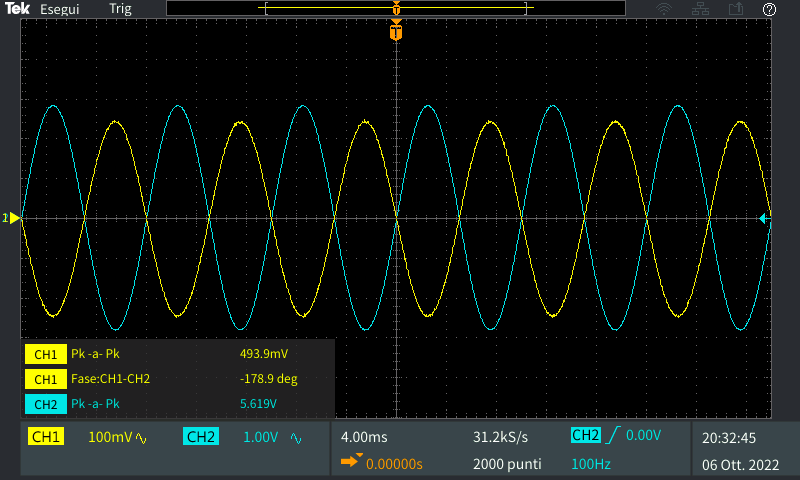
\includegraphics[width=0.8\linewidth]{./ImageFiles/Laboratorio 1/TEK00001}	
\end{figure}
\begin{figure}[h!]
	\centering
	b)
	
	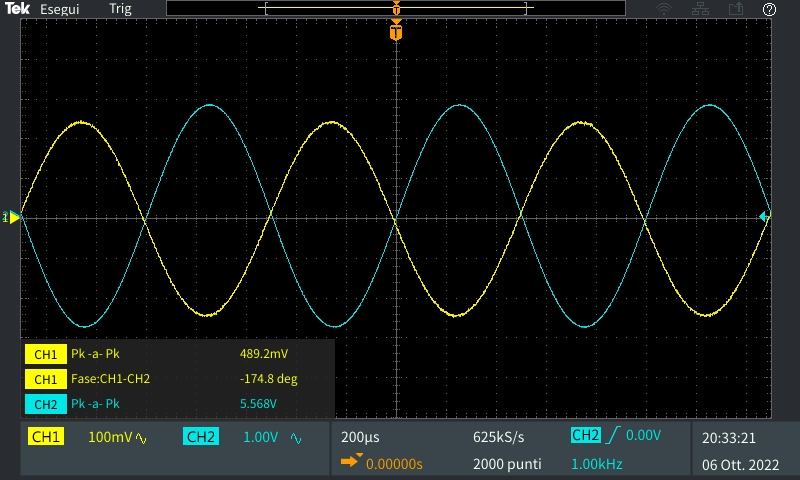
\includegraphics[width=0.8\linewidth]{./ImageFiles/Laboratorio 1/TEK00002}
\end{figure}
\begin{figure}[h]
	\centering
	c)
	
	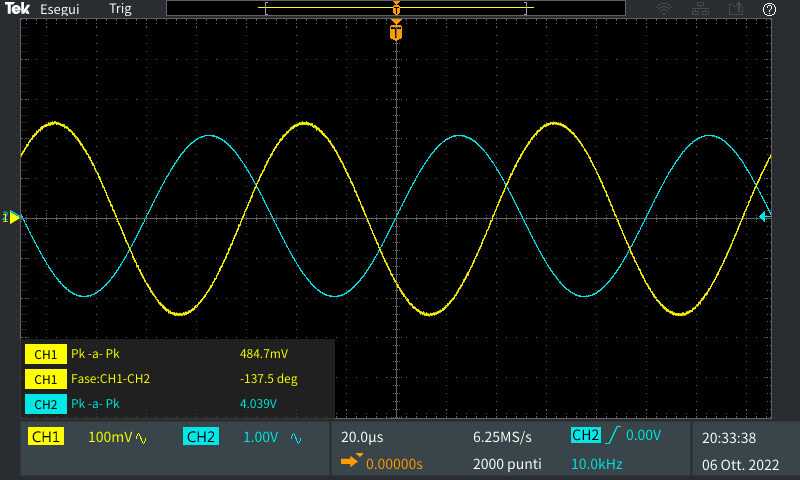
\includegraphics[width=0.8\linewidth]{./ImageFiles/Laboratorio 1/TEK00004}
	\caption{Misure del segnale in ingresso (linea gialla) e segnale in uscita (linea azzurra) al circuito. Si è utilizzato in ingresso un segnale sinusoidale con ampiezza picco-picco di \SI{500}{\milli\volt} e frequenza di \SI{100}{\hertz} (figura a), \SI{1}{\kilo\hertz} (figura b) e \SI{10}{\kilo\hertz} (figura c).}
	\label{fig:misure_oscilloscopio_1}
\end{figure}

\noindent
Tramite le funzioni fornite dall'oscilloscopio, sono state ottenute le misure di ampiezza picco-picco del segnale in uscita al circuito e la differenza di fase tra il segnale in ingresso e quello in uscita. Grazie a questi valori sono stati ricostruiti i diagrammi di Bode di modulo e fase del circuito, riportati in figura \ref{fig:diagrammi_di_Bode}.
\begin{figure}[h!]
	\centering
	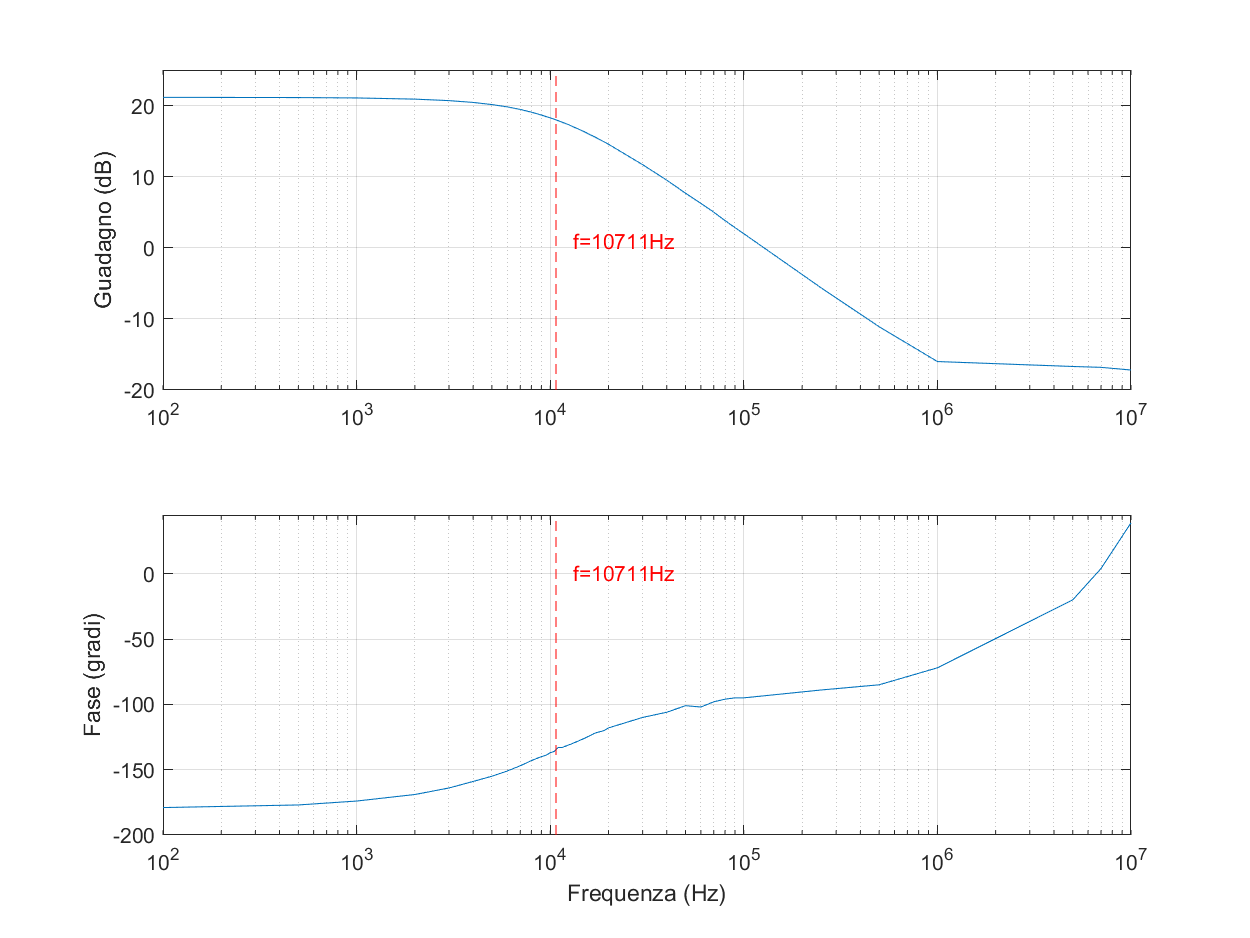
\includegraphics[width=0.80\linewidth]{./ImageFiles/Laboratorio 1/Diagrammi di Bode.png}
	\caption{Diagrammi di Bode del modulo e della fase del filtro realizzato.}
	\label{fig:diagrammi_di_Bode}
\end{figure}
Dai diagrammi di Bode della funzione di trasferimento si può osservare il comportamento del filtro passa basso. Osservando il modulo si può notare che fino alla frequenza di taglio, pari a \SI{10711}{\hertz}, il segnale in ingresso viene amplificato di circa \SI{20}{\decibel} (più precisamente il guadagno del circuito pari a 11.58, ossia \SI{21.27}{\decibel}), mentre per valori di frequenza superiori alla frequenza di taglio viene attenuato con una pendenza pari a \SI{20}{\decibel}/dec. Inoltre, osservando il diagramma della fase, si può notare che, in corrispondenza della frequenza di taglio, la fase è aumentata di circa 45$^{\circ}$ rispetto alle frequenza più basse, mentre fino a circa \SI{1}{\mega\hertz} tende a -90$^{\circ}$.
Tuttavia, per frequenze superiori a \SI{1}{\mega\hertz}, il comportamento del circuito non è più quello ideale descritto dalla formula \ref{eq:1.3}: infatti, a tali frequenze subentrano dei limiti e dei comportamenti in frequenza particolari causati dalla banda limitata di funzionamento dell'amplificatore operazionale.
\clearpage
In seguito, si è voluto analizzare il comportamento del circuito quando in ingresso si applica un segnale con ampiezza picco-picco crescente. I risultati sono mostrati nella figura \ref{fig:misure_oscilloscopio_sat}.
\begin{figure}[h!]
	\centering
	a)
	
	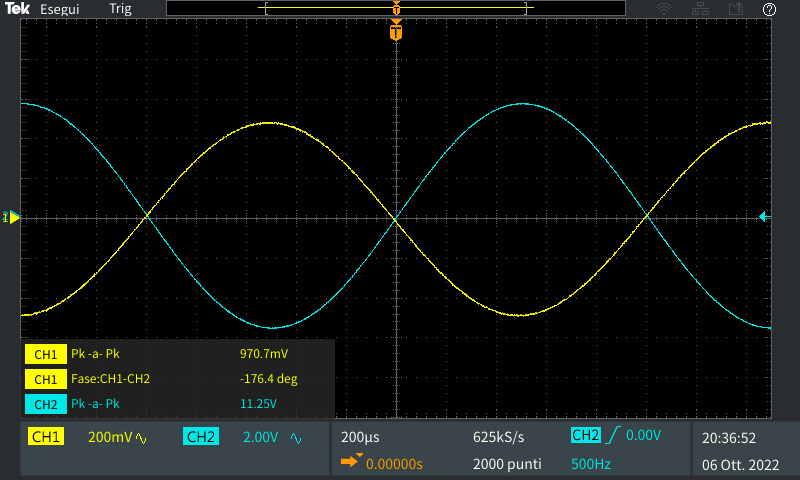
\includegraphics[width=0.8\linewidth]{./ImageFiles/Laboratorio 1/TEK00008}	
\end{figure}
\begin{figure}[h!]
	\centering
	b)
	
	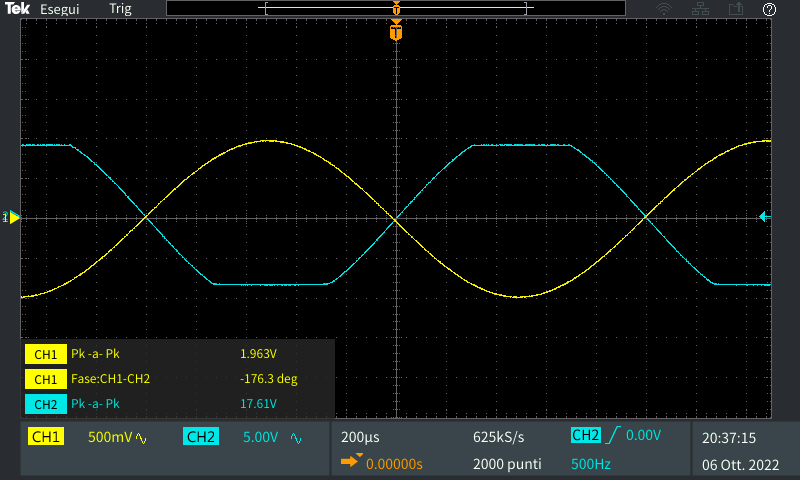
\includegraphics[width=0.8\linewidth]{./ImageFiles/Laboratorio 1/TEK00009}
\end{figure}
\begin{figure}[h!]
	\centering
	c)
	
	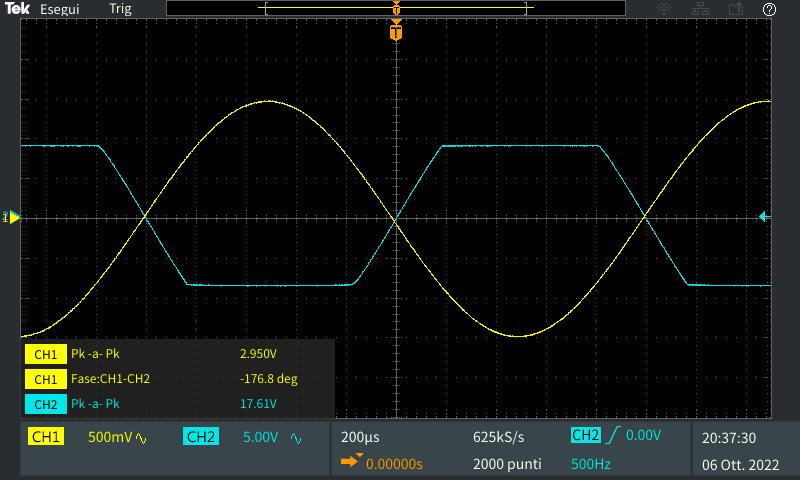
\includegraphics[width=0.8\linewidth]{./ImageFiles/Laboratorio 1/TEK00010}
	\caption{Misure del segnale in ingresso (linea gialla) e segnale in uscita (linea azzurra) al circuito. Si è utilizzato in ingresso un segnale sinusoidale con ampiezza picco-picco di circa \SI{1}{\volt} (figura a), \SI{2}{\volt} (figura b) e \SI{3}{\volt} (figura c) e con frequenza di \SI{500}{\hertz}.}
	\label{fig:misure_oscilloscopio_sat}
\end{figure} 

\newpage
\noindent
Come si può vedere nella figura \ref{fig:misure_oscilloscopio_sat}b, quando la sinusoide in ingresso ha una ampiezza di circa \SI{2}{\volt}, il segnale in uscita presenta una distorsione. Questo comportamento è descritto dal fenomeno di saturazione della tensione di uscita dell'amplificatore operazionale. Esso è caratterizzato da due fattori:
\begin{itemize}
	\item guadagno del circuito;
	\item tensioni di alimentazione positiva +E e negativa -E dell'amplificatore operazionale.
\end{itemize} 
Infatti, la tensione in uscita all'amplificatore operazionale (sul morsetto \textit{v\sub{out}}) non può assumere valori superiori alle tensioni di alimentazione del circuito, nel nostro caso fissate rispettivamente a +\SI{10}{\volt} e a -\SI{10}{\volt}. Dal momento che in ingresso è fornita un'onda sinusoidale di ampiezza picco-picco pari a \SI{2}{\volt} e considerando un fattore di guadagno di circa 11.6, il circuito dovrebbe presentare in uscita una sinusoide di ampiezza picco-picco di \SI{23}{\volt}, ossia una funzione sinusoidale che oscilla tra +\SI{11.5}{\volt} e -\SI{11.5}{\volt}. Questo però non è possibile perché significherebbe superare le tensioni di alimentazione del circuito e quindi l'uscita satura a valori pari alle alimentazioni. In realtà, a causa dei circuiti interni all'amplificatore operazionale, in un circuito reale l'uscita satura a tensioni inferiori a +E e superiori a -E (a meno che non si tratti di amplificatori \textit{rail-to-rail}, ma non è il caso del TL071). Inoltre, le tensioni di saturazione positiva e negativa possono assumere valori diversi, presentando un comportamento asimmetrico. Il fenomeno della saturazione diventa ancora più evidente nella figura \ref{fig:misure_oscilloscopio_sat}c, dove in ingresso viene applicato un segnale sinusoidale di ampiezza picco-picco di \SI{3}{\volt}.

\noindent
Dalle figure \ref{fig:misure_oscilloscopio_sat}b e \ref{fig:misure_oscilloscopio_sat}c  è possibile anche ricavare la massima ampiezza picco-picco che il segnale in uscita può assumere senza che si presenti il fenomeno della saturazione, misurando l'ampiezza picco-picco dei segnali saturati in uscita: in questo circuito tale valore è pari a \SI{17.61}{\volt}. Infatti, si può osservare che in figura \ref{fig:misure_oscilloscopio_sat}a il segnale in uscita non presenta distorsioni poiché il valore picco-picco è pari a \SI{11.25}{\volt}. 

\noindent
Per cercare di eliminare il fenomeno della saturazione si potrebbe pensare di aumentare le tensioni di alimentazione del circuito: così facendo si aumenta l'ampiezza massima possibile della sinusoide in uscita. Tuttavia, non è possibile aumentare a piacere il valore di queste tensioni. Infatti, è necessario verificare sul datasheet le tensioni massime sopportate dal particolare opamp. Oppure i limiti sulle tensioni applicabili sono definiti dai generatori utilizzabili nella particolare applicazione. Tipicamente, si cerca di mantenere le tensioni di alimentazione più basse possibili in modo da limitare i consumi del circuito.


Infine, si è analizzato il comportamento del circuito modificando la tensione di offset applicata al segnale in ingresso. Applicare una tensione di offset alla sinusoide in ingresso significa alzare la sinusoide rispetto alle prove eseguite fino ad ora (\Fig\ref{fig:misure_oscilloscopio_offset_sinusoide}).
\begin{figure}[h!]
	\centering
	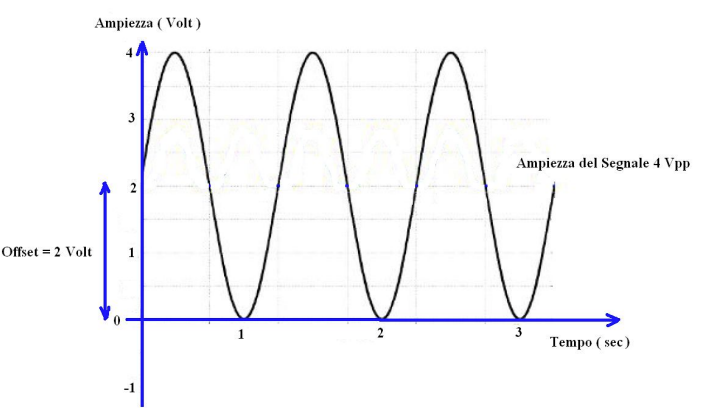
\includegraphics[width=0.6\linewidth]{./ImageFiles/Laboratorio 1/tensione offset}
	\caption{Illustrazione della tensione di offset di una sinusoide.}
	\label{fig:misure_oscilloscopio_offset_sinusoide}
\end{figure} 

\noindent
In figura \ref{fig:misure_oscilloscopio_offset} sono riportati i grafici dei segnali in ingresso ed in uscita al variare della tensione di offset.

\noindent
Dalle misure effettuate è possibile notare che il segnale in uscita presenta le seguenti caratteristiche:
\begin{itemize}
	\item fattore di amplificazione rispetto al segnale in ingresso pari al guadagno del circuito;
	\item fase di circa 180$^\circ$ rispetto al segnale in ingresso (amplificatore invertente);
	\item offset amplificato di un fattore pari al guadagno del circuito e di segno opposto rispetto all'offset del segnale in ingresso.
\end{itemize}
Da questi risultati si comprende che anche la parte DC del segnale in ingresso è soggetta ad un fattore di amplificazione pari a $-\frac{R_1}{R_2}$. Infatti, aumentando l'offset del segnale in uscita aumenta la differenza di potenziale ai capi della resistenza R\sub{2} e di conseguenza la corrente che ne scorre attraverso (legge di Ohm). Considerando nulle le correnti di ingresso all'amplificatore, aumenta la corrente anche in R\sub{1}. Tuttavia, dal momento che il nodo V\super{-} è una massa virtuale, è necessario che la tensione sul nodo V\sub{out} diminuisca. Per questo motivo, l'offset in uscita avrà segno opposto rispetto a quello in ingresso. Considerazioni analoghe possono essere fatte per offset negativi applicati in ingresso.
Anche in questi casi bisogna prestare attenzione a non far saturare l'uscita: infatti, se l'offset applicato in ingresso è troppo elevato, la sinusoide in uscita viene tagliata dalla saturazione dell'operazionale, come mostrato in figura \ref{fig:misure_oscilloscopio_offset_sat}. In particolare, si è notato un comportamento non simmetrico delle tensioni di saturazione: infatti, applicando un offset positivo di +\SI{500}{\milli\volt} il segnale in uscita raggiungeva la tensione di saturazione negativa. Al contrario, è necessario applicare un offset di -\SI{600}{\milli\volt} per raggiungere la tensione di saturazione positiva.

\begin{figure}[h]
	\centering
	a)
	
	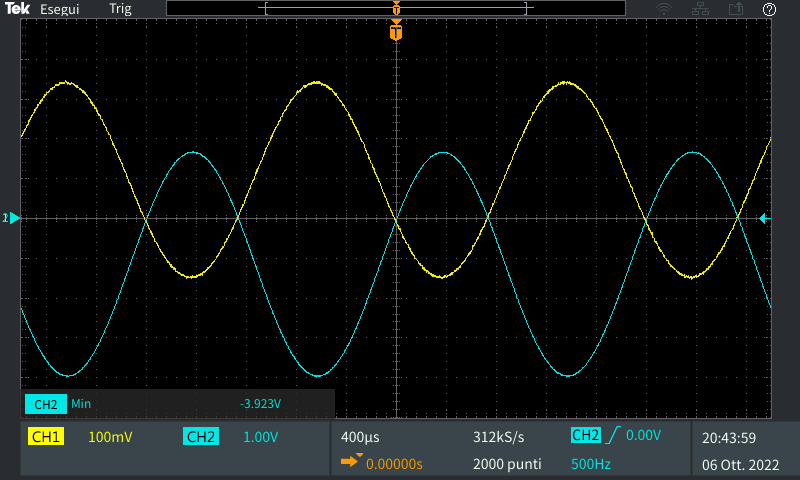
\includegraphics[width=0.8\linewidth]{./ImageFiles/Laboratorio 1/TEK00012}	
\end{figure}
\begin{figure}[h]
	\centering
	b)
	
	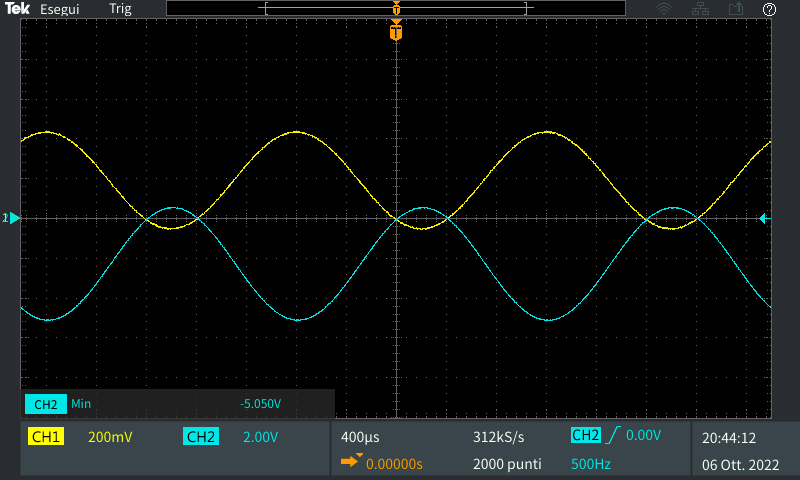
\includegraphics[width=0.8\linewidth]{./ImageFiles/Laboratorio 1/TEK00013}
\end{figure}
\begin{figure}[h]
	\centering
	c)
	
	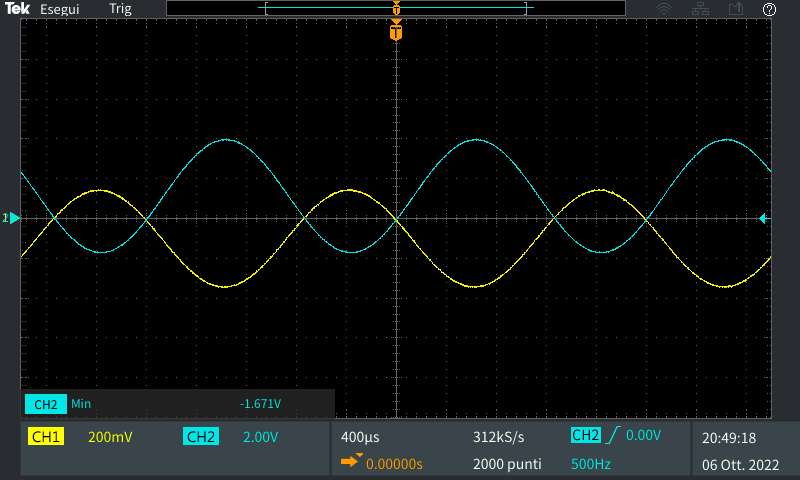
\includegraphics[width=0.8\linewidth]{./ImageFiles/Laboratorio 1/TEK00014}
\end{figure}
\begin{figure}[h]
	\centering
	d)
	
	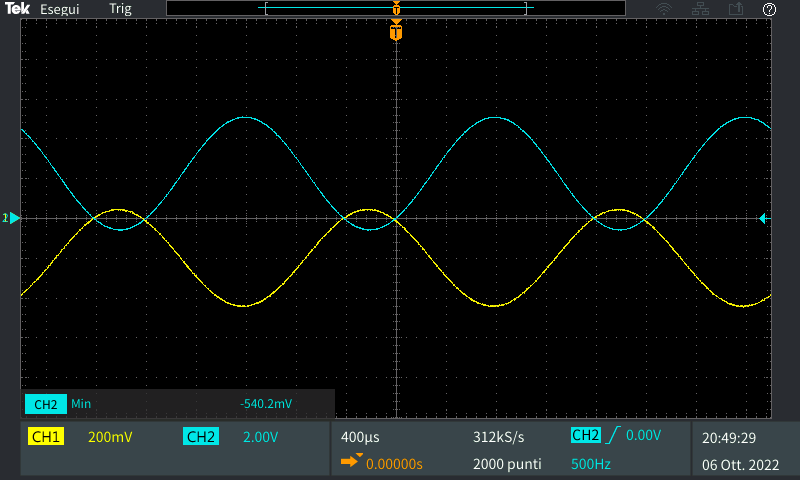
\includegraphics[width=0.8\linewidth]{./ImageFiles/Laboratorio 1/TEK00015}
	\caption{Misure del segnale in ingresso (linea gialla) e segnale in uscita (linea azzurra) al circuito. Si è utilizzato in ingresso un segnale sinusoidale con ampiezza picco-picco di \SI{500}{\milli\volt}, frequenza di \SI{500}{\hertz} e offset di +\SI{100}{\milli\volt} (figura a), +\SI{200}{\milli\volt} (figura b), -\SI{100}{\milli\volt} (figura c) e -\SI{200}{\milli\volt} (figura d).}
	\label{fig:misure_oscilloscopio_offset}
\end{figure} 

\begin{figure}[h]
	\centering	
	\begin{minipage}{.45\textwidth}
		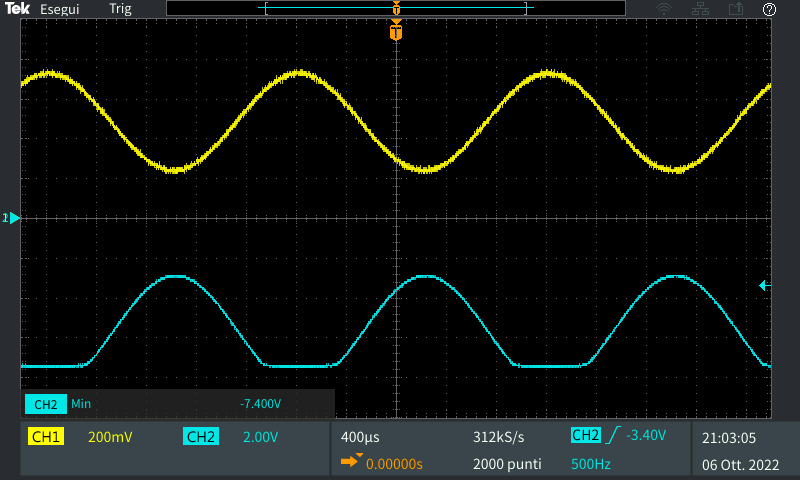
\includegraphics[width=\linewidth]{./ImageFiles/Laboratorio 1/TEK00019}
	\end{minipage}
	\qquad\qquad
	\begin{minipage}{.45\textwidth}
		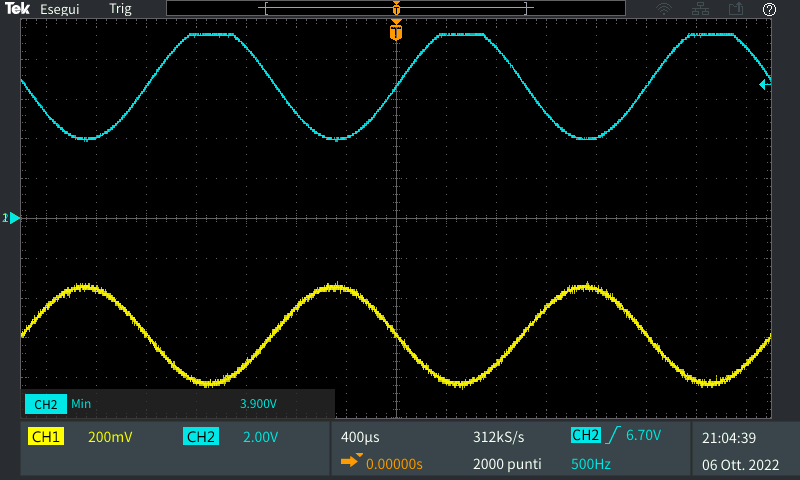
\includegraphics[width=\linewidth]{./ImageFiles/Laboratorio 1/TEK00021}
	\end{minipage}
	
	\caption{Misure del segnale in ingresso (linea gialla) e segnale in uscita (linea azzurra) al circuito. Si è utilizzato in ingresso un segnale sinusoidale con ampiezza picco-picco di \SI{500}{\milli\volt}, frequenza di \SI{500}{\hertz}.  A sinistra è stato applicato un offset di +\SI{500}{\milli\volt}, mentre a destra di -\SI{600}{\milli\volt}.}
	\label{fig:misure_oscilloscopio_offset_sat}
\end{figure}
